\documentclass[crop, tikz]{standalone}

\usepackage[utf8]{inputenc}
% 'crop' is the default for v1.0, before it was 'preview'
%\usetikzlibrary{...}% tikz package already loaded by 'tikz' option

\usetikzlibrary{arrows}
\usetikzlibrary{decorations.markings}

\begin{document}

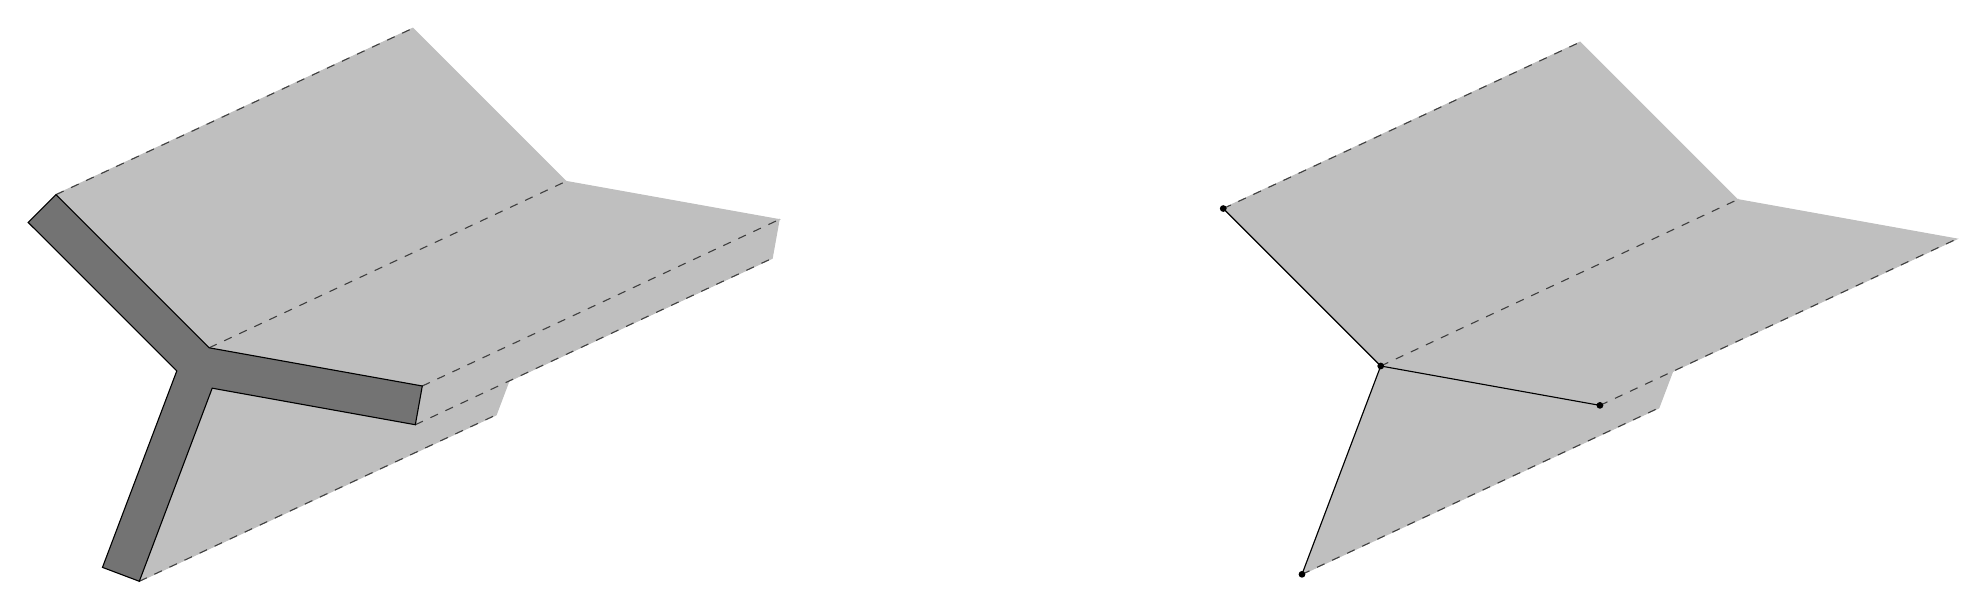
\begin{tikzpicture}

	%Graph in the 2D plane, place on the right ideally.
	\pgfdeclarelayer{foreground}
	\pgfdeclarelayer{background}
	\pgfsetlayers{background,main,foreground}

	%extruded graph
	\begin{scope}[shift={(15,0)}]
		\coordinate (centre) at (0,0);
		\coordinate (centrePlaneEnd) at (({5*cos(25)},{5*sin(25)});
		\coordinate (v1) at (-2,2);
		\coordinate (v1PlaneEnd) at ({5*cos(25) -2},{5*sin(25) +2});
		\coordinate (v2) at (-1,-{sqrt(8-1*1)});
		\coordinate (v2PlaneEnd) at ({5*cos(25)-1},{5*sin(25) -sqrt(8-1*1)});
		\coordinate (v3) at ({sqrt(8-0.5*0.5)},-0.5);
		\coordinate (v3PlaneEnd) at ({5*cos(25) + sqrt(8-0.5*0.5)},{-0.5+5*sin(25)});
		\begin{pgfonlayer}{foreground}
			%graph edges
			\draw (centre) -- (v1);
			\draw (centre) -- (v2);
			\draw (centre) -- (v3);
			%graph vertices
			\filldraw[black] (centre) circle (1pt);
			\filldraw[black] (v1) circle (1pt);
			\filldraw[black] (v2) circle (1pt);
			\filldraw[black] (v3) circle (1pt);
		\end{pgfonlayer}
		%extruded planes, draw planes coming out at an angle of 25 degrees, with length 5
		%plane outlines
		\draw[dashed, black!75!white] (centre) -- (centrePlaneEnd);
		\draw[dashed, black!75!white] (v1) -- (v1PlaneEnd);
		\draw[dashed, black!75!white] (v2) -- (v2PlaneEnd);
		\draw[dashed, black!75!white] (v3) -- (v3PlaneEnd);
		%plane fills
		\begin{pgfonlayer}{background}
			\filldraw[black!25!white] (centre) -- (centrePlaneEnd) -- (v1PlaneEnd) -- (v1) -- cycle;	
			\filldraw[black!25!white] (centre) -- (centrePlaneEnd) -- (v2PlaneEnd) -- (v2) -- cycle;	
			\filldraw[black!25!white] (centre) -- (centrePlaneEnd) -- (v3PlaneEnd) -- (v3) -- cycle;	
		\end{pgfonlayer}
	\end{scope}

	%extruded thin structure
	%the width of the thin-structure will be 0.5 (default Tikz unit), although we may want this labelled at a later date.
	%we will inherit the extrusion properties of the graph-portion of the diagram.
	\begin{scope}[shift={(0,0)}]
		\def\mag{0.25*sqrt(129)}
		\coordinate (origin) at (0,0);
		\coordinate (v1NE) at ({\mag*cos(135-5.051)},{\mag*sin(135-5.051)});
		\coordinate (v1SW) at ({\mag*cos(135+5.051)},{\mag*sin(135+5.051)});
		\coordinate (v2NW) at ({\mag*cos(180+69.3-5.051)},{\mag*sin(180+69.3-5.051)});
		\coordinate (v2SE) at ({\mag*cos(180+69.3+5.051)},{\mag*sin(180+69.3+5.051)});
		\coordinate (v3NE) at ({\mag*cos(360-10.18+5.051)},{\mag*sin(360-10.18+5.051)});
		\coordinate (v3SW) at ({\mag*cos(360-10.18-5.051)},{\mag*sin(360-10.18-5.051)});
		\coordinate (v1v2) at (-0.28980064668268024, -0.062379715847568074);
		\coordinate (v2v3) at (0.15974864250714188, -0.2817055447064405);
		\coordinate (v3v1) at (0.12087659909877639, 0.23130376343147308);
		\begin{pgfonlayer}{foreground}
			%2D-structure border
			\filldraw[black!55!white, draw=black] (v1SW) -- (v1v2) -- (v2NW) -- (v2SE) -- (v2v3) -- (v3SW) -- (v3NE) -- (v3v1) -- (v1NE) -- cycle;
		\end{pgfonlayer}
		%extruded planes, draw planes coming out at an angle of 25 degrees, with length 5
		%plane outlines
		\coordinate (v1NEPlaneEnd) at ({\mag*cos(135-5.051) + 5*cos(25)},{\mag*sin(135-5.051) + 5*sin(25)});
		\coordinate (v3v1PlaneEnd) at ({0.12087659909877639 + 5*cos(25)}, {0.23130376343147308 + 5*sin(25)});
		\coordinate (v3NEPlaneEnd) at ({\mag*cos(360-10.18+5.051)+ 5*cos(25)},{\mag*sin(360-10.18+5.051) + 5*sin(25)});
		\coordinate (v3SWPlaneEnd) at ({\mag*cos(360-10.18-5.051)+ 5*cos(25)},{\mag*sin(360-10.18-5.051) + 5*sin(25)});
		\coordinate (v2SEPlaneEnd) at ({\mag*cos(180+69.3+5.051) +5*cos(25)},{\mag*sin(180+69.3+5.051) + 5*sin(25)});
		\coordinate (v2v3PlaneEnd) at ({0.15974864250714188 +5*cos(25)}, {-0.2817055447064405 + 5*sin(25)});
		\draw[dashed, black!75!white] (v1NE) -- (v1NEPlaneEnd);
		\draw[dashed, black!75!white] (v3v1) -- (v3v1PlaneEnd);
		\draw[dashed, black!75!white] (v3NE) -- (v3NEPlaneEnd);
		\draw[dashed, black!75!white] (v3SW) -- (v3SWPlaneEnd);
		\draw[dashed, black!75!white] (v2SE) -- (v2SEPlaneEnd);
		%plane fills
		\begin{pgfonlayer}{background}
			\filldraw[black!25!white] (v1NE) -- (v1NEPlaneEnd) -- (v3v1PlaneEnd) -- (v3v1) -- cycle;
			\filldraw[black!25!white] (v3NE) -- (v3NEPlaneEnd) -- (v3v1PlaneEnd) -- (v3v1) -- cycle;
			\filldraw[black!25!white] (v2SE) -- (v2SEPlaneEnd) -- (v2v3PlaneEnd) -- (v2v3) -- cycle;
			\filldraw[black!25!white] (v3SW) -- (v3SWPlaneEnd) -- (v3NEPlaneEnd) -- (v3NE) -- cycle;
		\end{pgfonlayer}
	\end{scope}

\end{tikzpicture}

\end{document}